\subsection{Implementación SRGAN.}

La implementación de este modelo se realizara utilizando la arquitectura presentada
en \cite{SRGAN} mediante el lenguaje \emph{Python} utilizando la librería de alto nivel \emph{Keras}

Keras es una API que proporciona numerosos bloques
de construcción útiles los cuales pueden ser conectados para crear arquitecturas de
aprendizaje profundo altamente complejas.

Para el entrenamiento de las redes, Keras utiliza una de las tres librerías como
\emph{backend} para este propósito: \emph{TensorFlow}, \emph{CNTK}, o \emph{Theano}. Para esta implementación
se utiliza \emph{TensorFlow}, que es una librería de Python de código abierto para el
aprendizaje automático, esta fue desarrollada por Google.

Utilizaremos el dataset MIRFLICKR \cite{MIRFLICKR} el cual es una base de datos de imágenes
extraídas de la red social flickr, esta base consta de 25000 imágenes y la principal ventaja es 
que las imágenes son muy variadas por lo cual es ideal en el entrenamiento de una red neuronal capaz 
de mejorar los detalles de una imagen. Cabe resaltar que no se utilizaron todas las imágenes del dataset
debido al tiempo de ejecución del entrenamiento, así como las limitantes de hardware al ejecutar el código.

\subsubsection{VGG19.}

VGG19 (Visual Geometry Group) es la red convolucional pre-entrenado que se utilizara en el código
dedicada a la clasificación de imágenes ,consta de 16 capas convolucionales, 3 capas completamente conectadas, 5 capas de 
Maxpooling (Valores máximos de los parches)  y 1 capa de SoftMax como se observa en la imagen \ref{Alexis35}. El modelos se construyó
 con imagenet (base de datos) cuya salida son las características de la imagen extraídas en el tercer bloque de el modelo (pesos),
 esta red será la que utilizaremos durante el entrenamiento con el fin de optimizar el proceso del entrenamiento de la red
ya que sin el se saturaría el tiempo de ejecución.

 
\begin{figure}[H]
  \begin{center}
    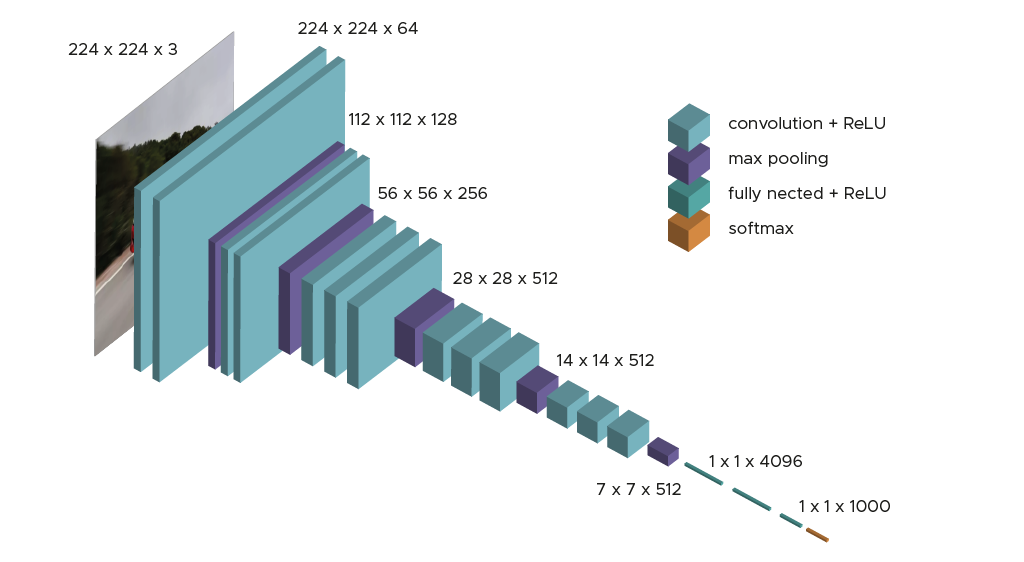
\includegraphics[scale = 0.4]{VGG19.png}
    \caption{Arquitectura de la red VGG19}
    \label{Alexis35}
  \end{center}
\end{figure}


\subsubsection{Modelo generador.}

Las imágenes originales del dataset son de una dimensión de 500x500 pixeles, para el modelo generador
se utiliza una imagen de entrada de baja resolución de 32x32 pixeles y la imagen de alta resolución de salida
será de 128x128 pixeles, teniendo un escalado de 4 veces el tamaño original, algunas de estas imágenes pueden
visualizarse en la imagen \ref{fig:fr_dataset}.


Se comienza a crear el modelo generador utilizando bloques de
redes residuales (Las redes residuales o ResNet fueron
propuestas en 2015 por He et al. \cite{Resnet}), su finalidad es evitar el problema del desvanecimiento del gradiente. Así, la particularidad
que tienen las ResNet es que establecen conexiones salteándose algunas
capas como se puede ver en la figura \ref{Alexis4}.

Cada bloque de redes residuales se compone por dos redes convolucionales
seguidas por una capa de normalización por lotes. Finalmente, hay una
capa de adición que calcula la suma de la entrada al bloque y la salida
de la última capa de normalización. Se utiliza la función de activación, que nos ayuda a indicar cuando
se enciendo o apaga la neurona. En este modelo utilizamos la función 
PReLu (Parametric ReLu) con la cual multiplica cualquier valor negativo de la neurona
por un valor pequeño aproximado a 0.


El bloque de upsampling es el que nos ayudara a realizar el escalado de la imagen conforme al entrenamiento,
se encarga de realizar un aumento de pixeles mediante interpolaciones de vecino cercano para cada 
capa de convolución lo que se interpreta en un suavizado de la imagen y así mismo un aumento de tamaño.

La arquitectura completa del modelo generador se puede ver en la imagen \ref{Alexis4}.


\begin{figure}[H]
  \begin{center}
    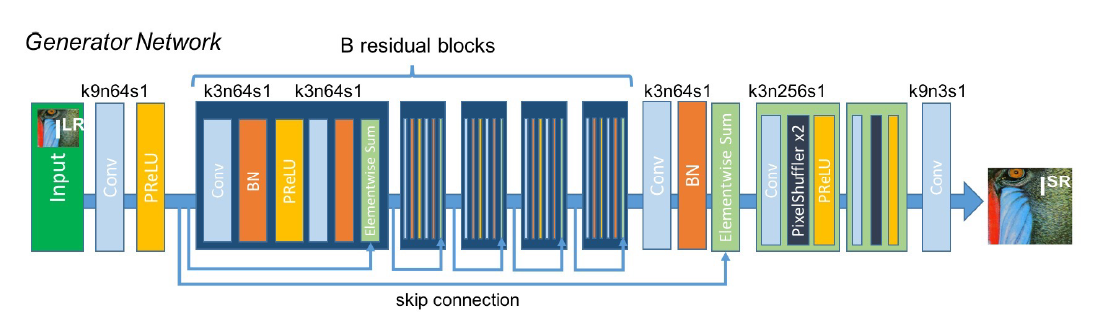
\includegraphics[scale = 0.7]{Imp_generador.png}
    \caption{Arquitectura del generador de la SRGAN,\emph{k} es el tamaño del
    filtro, \emph{n} es la dimensión del mapa de características (capa de convolución) y \emph{s} indica
    el valor del parámetro stride. Imagen tomada de \cite{SRGAN}}
    \label{Alexis4}
  \end{center}
\end{figure}

\subsubsection{Modelo discriminador.}

El modelo discriminador se asemeja mucho en la parte de la red neuronal a la arquitectura del modelo generador,
pero varia en la función de activación el cual estima un valor cercano a 0 que no depende de la red neuronal como tal, sino que
es constante además de esto, tenemos que la salida de este modelo es una probabilidad de que la imagen del modelo generador sea tomada
como una real y a partir de esto clasificarla como un 1 o u 0 (Clasificador Binario) es por esto que nuestra salida es una función 
\emph{Sigmoide}, ya que abarca valores de 0 a 1.

La arquitectura completa del modelo Discriminador se puede ver en la imagen \ref{Alexis5}.

\begin{figure}[H]
  \begin{center}
    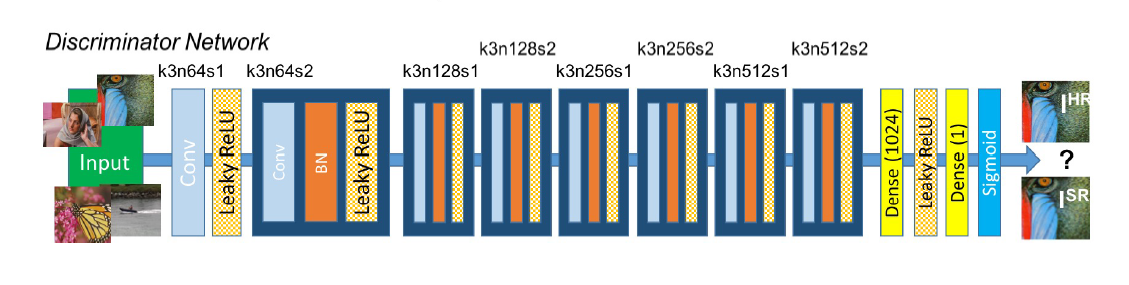
\includegraphics[scale = 0.7]{Imp_discriminador.png}
    \caption{Arquitectura del Discriminador de la SRGAN, \emph{k} es el tamaño
    del filtro, \emph{n} es la dimensión del mapa de características (capa de convolución) y \emph{s}
    indica el valor del parámetro stride. Imagen tomada de \cite{SRGAN}}
    \label{Alexis5}
  \end{center}
\end{figure}

\subsubsection{Entrenamiento}

EL modelo de entrenamiento de las GAN´s como se ha mencionado en \cite{GANs} y \cite{SRGAN}, es un proceso en el cual
los dos modelos compiten, el generador por engañar al discriminador y el discriminador por no permitirlo, en la figura \ref{Alexis6}
podemos ver este proceso.

\begin{figure}[H]
    \begin{center}
      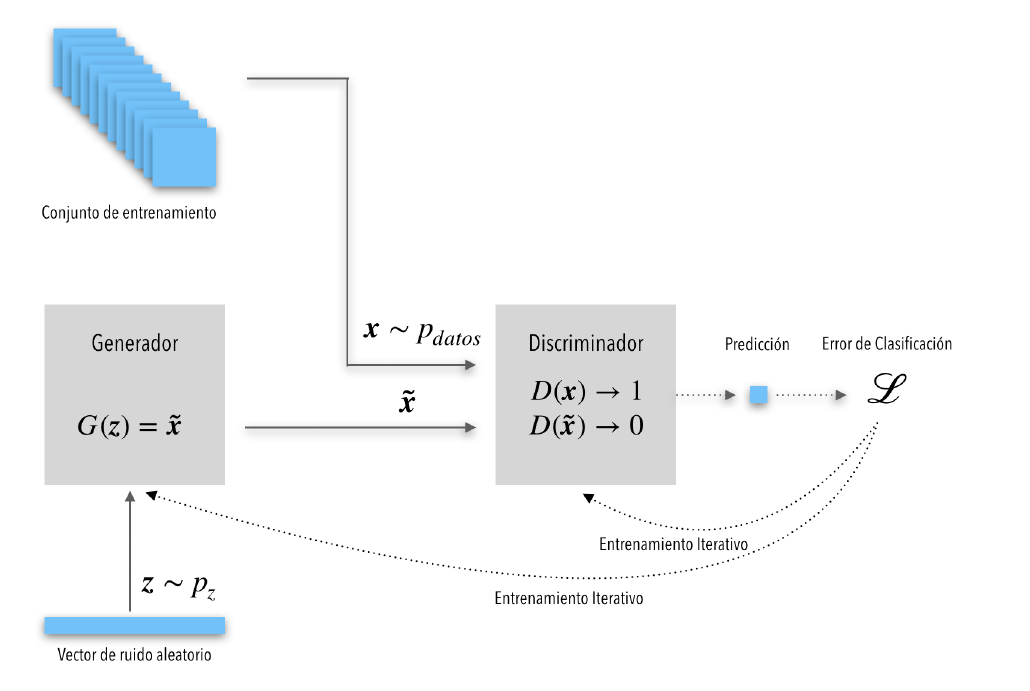
\includegraphics[scale = 0.6]{proceso_gan.png}
      \caption{Proceso de entrenamiento}
      \label{Alexis6}
    \end{center}
\end{figure}

Con la implementación del código en \emph{python} dadas las arquitecturas de ambos modelos (Generador y discriminador) 
se realiza un entrenamiento de la red GAN el cual se basa en obtener los Batches de imágenes los cuales son el conjunto
de datos utilizados por cada iteración dado un numero concreto de imágenes y un numero d épocas que no son mas que los ciclos
del algoritmo donde los datos pasan por la red neuronal. Se utiliza el optimizador Adam, antes descrito y la función \emph{Binary Crossentropy}
la cual se encarga de obtener las perdidas basándose en la clasificación del discriminador.

Después de realizar las épocas de entrenamiento se puede apreciar que a mayor numero de imágenes y 
épocas los resultados suelen ser mejores sobre todo para imágenes que no están en el dataset,en la imagen
\ref{Alexis7} podemos observar la mejora que se obtiene con 200 épocas de entrenamiento para tan solo 13 imágenes 
aun así la reconstrucción es buena y se logran percibir algunos detalles.

\begin{figure}[H]
  \begin{center}
    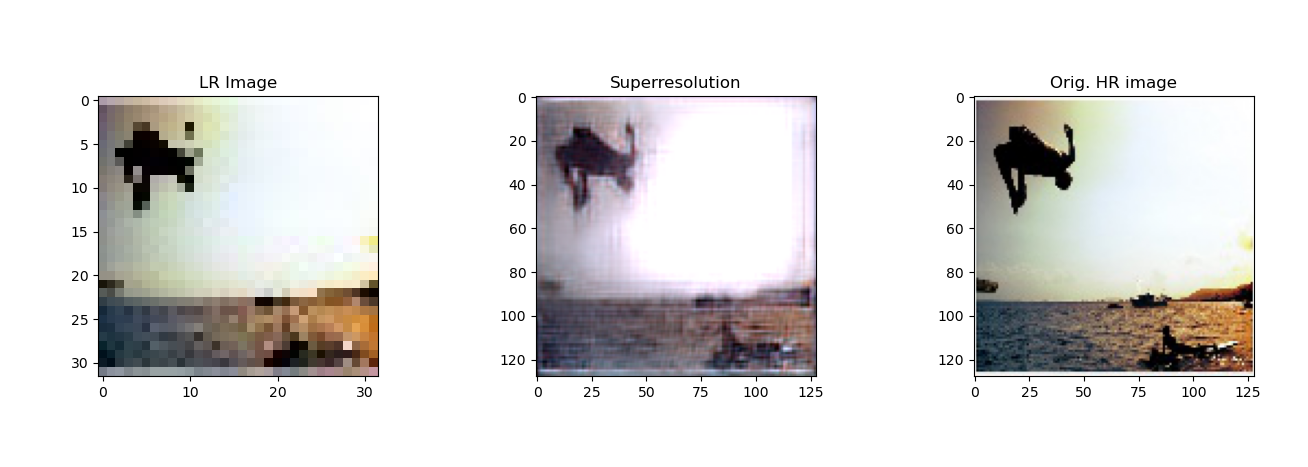
\includegraphics[scale = 0.4]{13im_200E.png}
    \caption{Imagen obtenida de un modelo generador de 200 épocas y 13 imágenes.}
    \label{Alexis7}
  \end{center}
\end{figure}

Conforme se aumentan las épocas de entrenamiento y el número de imágenes se comprueba
que los resultados son mejores como se observa en la imagen \ref{Alexis8} donde se aumentan
las épocas a 400 y el numero de imágenes a 50, con lo que podemos obtener mas detalles en nuestro modelo
gracias a al diversidad en estas imágenes.

\begin{figure}[H]
  \begin{center}
    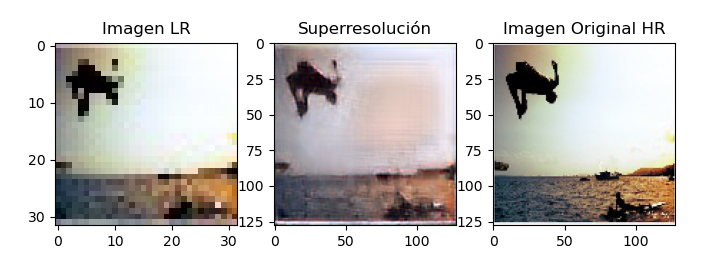
\includegraphics[scale = 0.9]{50im_400E.png}
    \caption{Imagen obtenida de un modelo generador de 400 épocas y 50 imágenes.}
    \label{Alexis8}
  \end{center}
\end{figure}

Una solución a este problema es realizar la carga del modelo generador antes del entrenamiento,
con esto el modelo generador toma la configuración de pesos y métricas anteriores y realiza el entrenamiento
a partir de estas, esto puede generar una mejora como se observa en la imagen \ref{Alexis9}, pero
también puede causar distorsión en el modelo que obtengamos como resultado, dada la interpretación del generador,
incluso se puede aumentar la perdida.

\begin{figure}[H]
  \begin{center}
    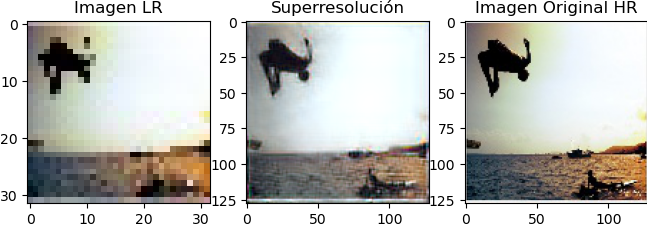
\includegraphics[scale = 0.57]{1000im_5E_Reentrenado.png}
    \caption{Imagen obtenida de un modelo generador entrenado a partir de 400 épocas y 50 imágenes cargado
    en el programa y luego entrenado a 5 épocas y 1000 imágenes.}
    \label{Alexis9}
  \end{center}
\end{figure}




\subsubsection{Métricas}

 Durante el entrenamiento podemos observar el tiempo que tarda nuestra red en realizar el entrenamiento, aunado a eso 
 podemos medir las perdidas de los modelos, dados los antecedentes, se tiene que las perdidas nos relacionan la mejora de la imagen
 a menor valor de perdida exista, mejor será la calidad del modelo generador, para el modelo discriminador ocurre lo mismo,
 entre menor sea el número, mejor podrá discernir entre una imagen generada y una real.

 Finalmente se puede observar que la Precisión del modelo generador tiende a un valor de 1,(100\%) esto quiere decir que
 en esa época sabrá discernir perfectamente una imagen de la otra, forzando al generador a tener menos perdida. Esto puede observarse en las
 gráficas de la imagen \ref{Alexis10}.

 \begin{table}[H]
  \centering
  \caption{Resultados Máximo y Mínimos de las perdidas.}
  \begin{tabular}{|l|l|l|}
  \hline
  \textbf{Criterio} & \textbf{Valor Máximo} & \textbf{Valor Mínimo}  \\ \hline
  Pérdida del Generador           & 228.5551261019351              & 23.898190839255033     \\
  Pérdida del Discriminador       & 1.236285184701566              & 1.6890162633455543e-16  \\
  Precisión Discriminador         & 1.0                            & 0.8630597014925373       \\ \hline
  \end{tabular}
\end{table}



\begin{figure}[H]
  \begin{center}
    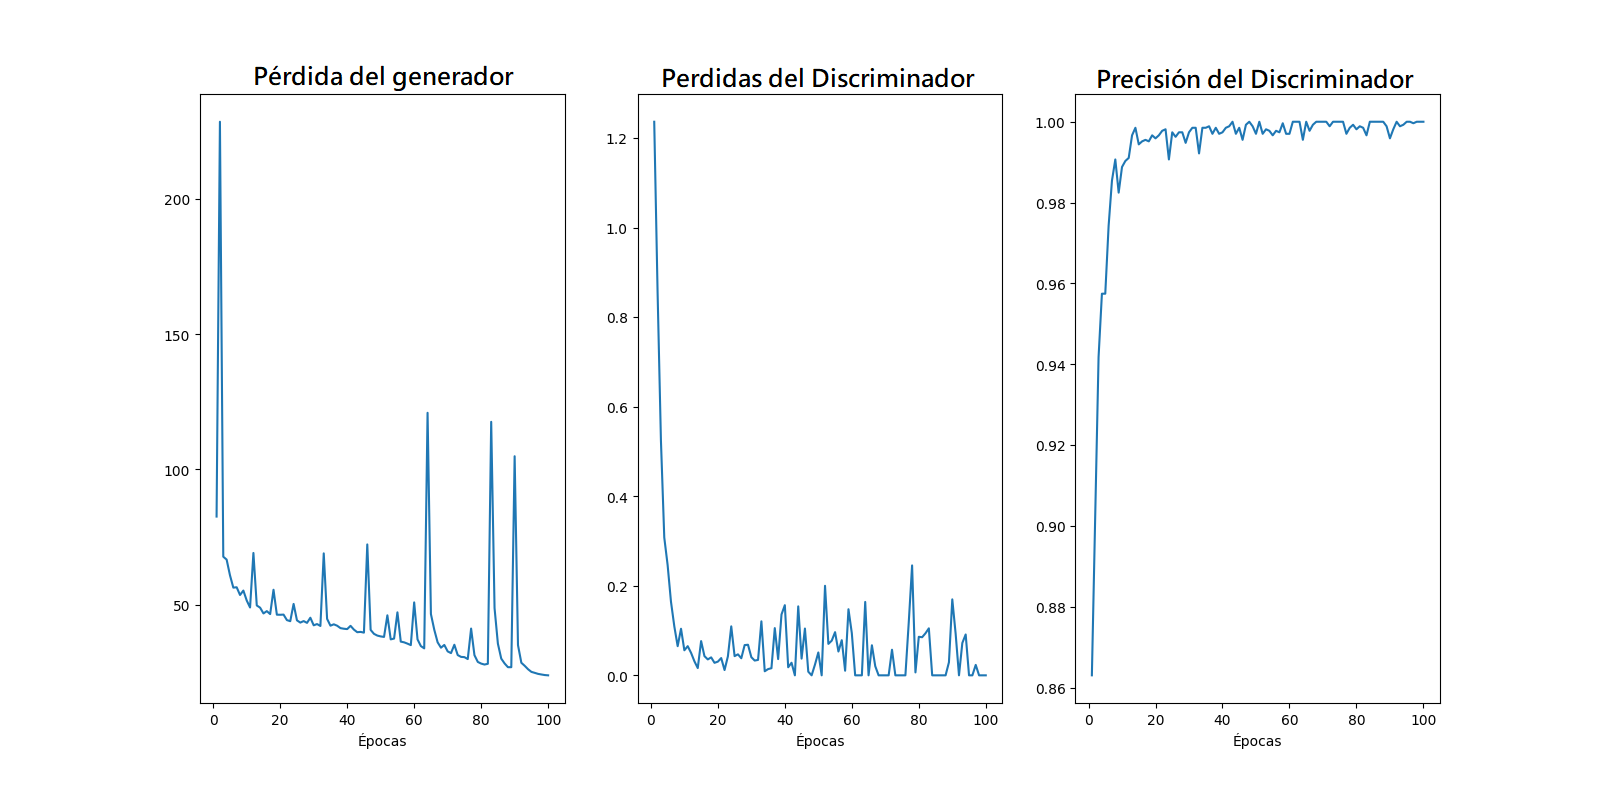
\includegraphics[scale = 0.6]{Graficasperdidas.png}
    \caption{Resultados de las perdidas durante el entrenamiento (2000 imágenes, 100 épocas)}
    \label{Alexis10}
  \end{center}
\end{figure}